\section{Binary to BCD Conversion}
\subsection{Aim}
To convert a binary number to BCD

\subsection{Code}
\begin{lstlisting}
DATA SEGMENT
  bin EQU 1000b
  result DW ?
DATA ENDS

CODE SEGMENT
ASSUME CS:CODE, DS:DATA
START:
  MOV AX, DATA
  MOV DS, AX
  MOV BX, bin
  XOR AX, AX
  XOR CX, CX

CONVLOOP:
  CMP BX, 0
  JE EXIT
  DEC BX
  MOV AL, CL
  ADD AL, 01H
  DAA
  MOV CL, AL
  MOV AL, CH
  ADC AL, 00H
  DAA
  MOV CH, AL
  JMP CONVLOOP

EXIT:
  MOV result, CX
  MOV AX, 4CH
  INT 21H
CODE ENDS
END START
\end{lstlisting}

\subsection{Output}
\begin{center}
	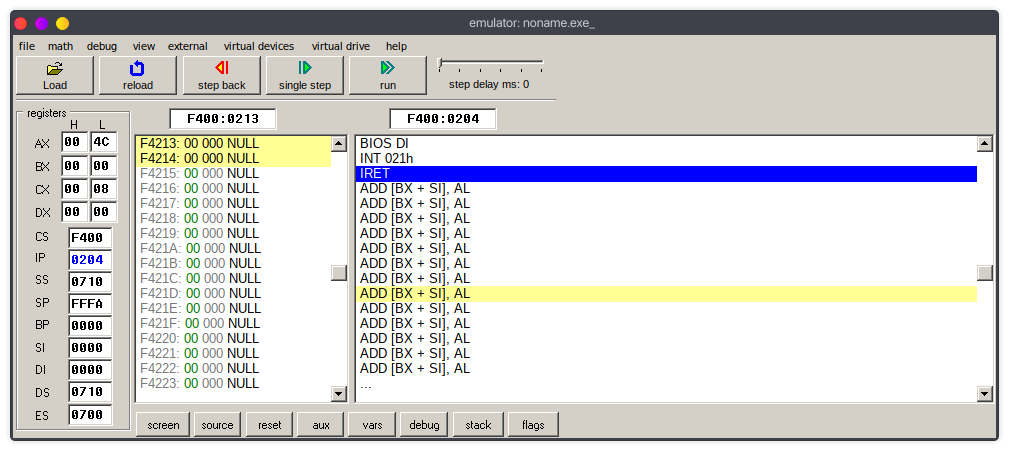
\includegraphics[width=0.90\textwidth]{img/p12/ss1.png}
	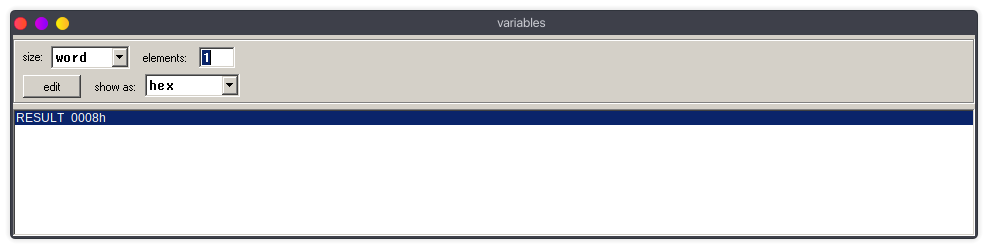
\includegraphics[width=0.90\textwidth]{img/p12/ss2.png}
\end{center}

\subsection{Result}
A binary number was converted to BCD in emu8086